\documentclass[10pt,a4paper]{article}
\usepackage[margin=1.5cm]{geometry}
\usepackage{amsmath,amssymb}
\usepackage{graphicx}
\usepackage{booktabs,tabularx}
\usepackage{xcolor}
\usepackage{enumitem}
\usepackage[numbers]{natbib}
\usepackage{hyperref}
\usepackage{float}
\usepackage{titlesec}
\hypersetup{colorlinks=true,linkcolor=blue!50!black,citecolor=blue!50!black,urlcolor=blue!50!black}
\setlist{itemsep=0.5pt,topsep=2pt}
\setlength{\emergencystretch}{1.5em}
\setlength{\parskip}{1pt}
\setlength{\textfloatsep}{7pt}
\setlength{\intextsep}{6pt}
\titleformat{\section}{\normalfont\large\bfseries}{\thesection.}{0.55em}{}
\titleformat{\subsection}{\normalfont\normalsize\bfseries}{\thesubsection.}{0.5em}{}
\newcolumntype{Y}{>{\raggedright\arraybackslash}X}
\title{\textbf{Exploring Temporal Degradation Patterns for Turbofan Engine Remaining Useful Life (RUL) Prediction.}\\[4pt]\large DS5006 Machine Learning --- Team Project Report}
\author{Team Afterburner\\[3pt]\small Rajorshi Adhikary (142602017) \quad Anesu Kabuku (142602026)\\\small Tanmoy Paul (142602020)}
\date{November 2026}
\begin{document}
\maketitle

\begin{abstract}
Remaining Useful Life (RUL) prediction from turbofan sensors is complicated by measurement noise, degradation and operating-regime changes. Using NASA C-MAPSS FD001 and FD002, we investigate whether temporal order adds information beyond window summaries (Q1), and whether operating-condition adjustment and its order improve prediction (Q2). For Q1, we compare current-cycle values, unordered window statistics, ordered trend features, and trend features after within-window shuffling. Random Forest, XGBoost, AdaBoost, Ridge and Lasso are evaluated in Q1 over window lengths of 5--50 cycles with engine-wise five-fold validation. At 50 cycles, ordered features reduce cross-validation RMSE over summary-only features by 4.2--4.4 cycles on FD001 and 5.8--6.3 cycles on FD002. Ridge and Lasso show the same qualitative preference for ordered features. For Q2, global normalization (N), adjustment before feature extraction (AF), and differencing before adjustment (DF) are compared at 50 cycles. On FD002, AF reduces validation RMSE from 23.05 to 14.04 for Random Forest, 22.97 to 13.81 for XGBoost, and 24.76 to 16.13 for AdaBoost. FD001 shows effectively no change, as expected for its single operating condition. Thus, temporal order helps at longer windows, while condition-aware adjustment has the largest effect in the multi-regime subset.
\end{abstract}

\section{Introduction and scientific questions:}
Predictive maintenance estimates the remaining operating life of equipment before failure. Turbofan sensor measurements reflect gradual degradation, operating-regime changes and measurement variability; a useful RUL model must distinguish these effects. Using NASA C-MAPSS, we study whether recent sensor order adds information beyond window summaries (Q1), and whether operating-condition adjustment improves prediction and depends on whether it is applied before or after temporal differencing (Q2).

\begin{description}[leftmargin=1.2em,style=nextline]
\item[Q1.] \textbf{Does the order of readings inside a window matter?}\\
\textbf{Hypothesis:} Most of the benefit of using history comes from noise reduction through aggregation; trend information adds a smaller benefit, expected mainly near failure and with longer windows, as stated in the approved proposal.\\
\textbf{Falsified if:} Shuffled-window features perform comparably to features computed in true temporal order, or the ordered representation does not improve on summary statistics.
\item[Q2.] \textbf{Does removing the effect of operating conditions help, and does it matter when we do it?}\\
\textbf{Hypothesis:} In FD002, condition-specific adjustment should improve prediction, and adjusting each observation before computing temporal features (AF) should outperform differencing raw observations before adjustment (DF). In FD001, which has one operating condition, adjustment should have little or no effect.\\
\textbf{Falsified if:} Adjustment does not materially improve FD002, AF does not outperform DF, or FD001 changes substantially despite having one regime.
\end{description}

\section{Related work:}
Saxena et al. introduced C-MAPSS as a simulated run-to-failure benchmark for turbofan prognostics \cite{saxena2008}. Subsequent studies have used recurrent and convolutional networks, support-vector regression, tree ensembles and hybrid attention models. Asif et al. highlight preprocessing and degradation-oriented sensor analysis for C-MAPSS \cite{asif2022}; recent work also explores pretrained time-series representations for RUL prediction \cite{dinten2025}. Our contribution is a controlled ablation of temporal order (Q1) and operating-condition adjustment order (Q2), using fixed classical model families to isolate representation effects.

\section{Data:}
We use the NASA Prognostics Center of Excellence (PCoE) Turbofan Engine Degradation Simulation dataset, specifically the FD001 and FD002 subsets \cite{cmapssdataset,saxena2008}. The dataset is distributed through NASA's PCoE Data Set Repository. Each row contains engine ID, cycle, three operating settings and 21 sensor measurements (26 columns). Training trajectories run to failure; official test trajectories are truncated and accompanied by final-cycle RUL labels. FD001 has one operating condition and FD002 has six; both represent high-pressure-compressor degradation. The supplied proposal does not specify a dataset licence, so none is asserted here.

\begin{table}[H]\centering
\caption{C-MAPSS subsets used in this project.}\begin{tabular}{lrr}\toprule
Property & FD001 & FD002\\\midrule
Training engines & 100 & 260\\
Training rows & 20,631 & 53,759\\
Official test engines & 100 & 259\\
Official test rows & 13,096 & 33,991\\
Operating conditions & 1 & 6\\
Fault modes & 1 & 1\\
Sensor variables & 21 & 21\\
Raw columns per row & 26 & 26\\\bottomrule\end{tabular}\end{table}

For training engine $i$, the uncapped target is the number of cycles remaining until failure, $RUL_{i,t}=T_i-t$. We use the capped target $y_{i,t}=\min(T_i-t,125)$; the same cap is applied to official test labels. Audits found no missing cells or duplicate engine-cycle rows; uncapped training RUL ranged from 0--361 (FD001) and 0--377 (FD002). The official test predicts once per engine at its final observed cycle. Validation folds are grouped by engine to prevent correlated cycles from the same trajectory entering both partitions.

\section{Methodology:}
\subsection{Temporal windows and feature construction:}
A trailing window at cycle $t$ contains observations $t-L+1,\ldots,t$ only. For each sensor, the unordered summary contains mean, standard deviation, minimum, maximum and median; the ordered representation adds linear slope, last-minus-first change, standard deviation of first differences and mean absolute first difference.
For sensor readings $x_1,\ldots,x_L$ in chronological order, the least-squares slope and first differences are
\[
\beta=\frac{\sum_{j=1}^{L}(j-\bar j)(x_j-\bar x)}{\sum_{j=1}^{L}(j-\bar j)^2},\qquad \Delta x_j=x_j-x_{j-1}.
\]
The remaining descriptors are $x_L-x_1$, $SD(\Delta x)$ and $MAD_{\Delta}=(L-1)^{-1}\sum_{j=2}^{L}|\Delta x_j|$. All use only the trailing window; no future observation is used.

For Q1, four feature conditions are constructed from the same trailing sensor history. They are deliberately nested: A uses only the current observation; B adds historical information but removes chronological ordering through summary statistics; C adds descriptors calculated from the true chronological sequence; and D repeats C after permuting the observations within each window. This design separates the value of having history (A versus B) from the additional value of preserving its order (B versus C), while C versus D checks whether the temporal descriptors depend on the true sequence rather than an arbitrary ordering. Condition A is a current-cycle baseline ($L=1$); B--D use the specified trailing window lengths $L\in\{5,10,20,30,50\}$.

\begin{table}[H]\centering\small
\caption{Q1 experimental conditions and the information retained or disrupted.}
\begin{tabularx}{\linewidth}{@{}l l Y Y@{}}\toprule
Condition & Representation & Construction & Scientific role / key comparison\\\midrule
A & Current-cycle baseline & The 21 sensor readings at the current cycle only; no earlier cycles are aggregated ($L=1$). & Reference point for asking whether adding recent history helps.\\
B & Unordered window summaries & For each selected sensor, calculate mean, standard deviation, minimum, maximum and median over the trailing $L$ cycles. & Adds historical context while discarding the order of observations; compare B with A.\\
C & Ordered temporal representation & Retain B's summary descriptors and add chronological slope, last-minus-first change, standard deviation of first differences and mean absolute first difference. & Tests whether temporal direction and local change add information beyond summaries; compare C with B.\\
D & Shuffled-order control & Within each trailing window, randomly permute the readings and recompute the temporal descriptors using the permuted sequence; retain the same feature definitions as C. & Tests whether C's gain relies on the true chronology; compare C with D.\\\bottomrule
\end{tabularx}
\end{table}

The conditions are not four different datasets or four different prediction targets. They are alternative representations of the same engine history, evaluated against the same capped RUL target. For B, C and D, the window length is varied over five values; A remains the current-cycle reference. The primary interpretation is therefore: A--B measures the contribution of historical aggregation, B--C measures the incremental contribution of ordered temporal descriptors, and C--D measures sensitivity to destroying the true within-window order. Shuffling is a diagnostic control, not a physically realistic degradation trajectory.

For Q2, the feature representation is fixed to the ordered feature set and $L=50$. The experiment report specifies 19 selected sensor variables for FD001 and 21 for FD002 (171 and 189 descriptors, respectively). Training windows are sampled with stride four to reduce redundant overlap; validation scores every eligible cycle from cycle 50 onward. For official test evaluation, the final 50 observations are used. When a test trajectory has fewer than 50 observations, its first observation is repeated to left-pad the window; padded temporal differences are set to zero. Seven FD001 and 24 FD002 test engines require this padding.

\subsection{Operating-condition strategies:}
Q2 isolates the effect of operating-regime adjustment while keeping the temporal representation fixed. Regimes are assigned from the three operating settings using K-means after standardizing those settings. The number of regimes reflects the subset: FD001 has one operating condition, whereas FD002 has six. Regime assignment and sensor statistics are estimated from the training portion of each fold and then applied to its validation portion; for the official test set, they are fitted on the full training set and reused without refitting.

\begin{table}[H]\centering\small
\caption{Q2 preprocessing strategies: exact operation order and intended comparison.}
\begin{tabularx}{\linewidth}{@{}l l Y Y@{}}\toprule
Strategy & Short name & Processing sequence & What the comparison tests\\\midrule
N & Global normalization & For each sensor, subtract one global training-set mean and divide by one global training-set standard deviation. No regime-specific sensor scaling is applied. & Baseline that does not explicitly remove sensor shifts across operating regimes.\\
AF & Adjust first & (1) Assign each observation to an operating regime. (2) Normalize each sensor using the mean and standard deviation estimated for that regime from training data. (3) Construct the $L=50$ temporal windows and ordered features from the adjusted sensor levels. & Tests whether regime-specific adjustment before feature extraction makes sensor trajectories more comparable across operating conditions.\\
DF & Difference first & (1) Compute raw within-engine first differences. (2) Scale each difference by the standard deviation of the later observation's assigned regime. (3) Retain condition-normalized sensor levels for level-summary descriptors and construct the ordered feature representation. Differences at engine boundaries are set to zero. & Tests whether differencing before regime-specific scaling can remove operating-regime effects as effectively as adjusting sensor levels first.\\\bottomrule
\end{tabularx}
\end{table}

AF and DF are not interchangeable. AF transforms each observation into its regime-adjusted level before calculating temporal changes. DF calculates changes in the original sensor scale first and only then scales each difference using the later observation's regime scale. If a transition between regimes creates an offset in the raw sensor levels, scaling the raw difference does not necessarily remove that offset. N, AF and DF are compared using the same ordered feature representation and fixed window length $L=50$; unlike Q1, Q2 does not vary the feature condition or window length.

For observation $t$, sensor $s$, and assigned regime $k(t)$, the AF transformation is
\[
z^{AF}_{i,t,s}=\frac{x_{i,t,s}-\mu_{k(t),s}}{\sigma_{k(t),s}},
\]
where $\mu_{k,s}$ and $\sigma_{k,s}$ are estimated from training observations assigned to regime $k$. In DF, the raw within-engine difference is formed first and scaled using the later observation's regime scale, $\Delta x_{i,t,s}/\sigma_{k(t),s}$; this does not in general remove a regime offset in the raw difference.

\subsection{Regression models:}
The Q1 comparison includes five model families: Random Forest (RF), XGBoost (XGB), AdaBoost (ADA), Ridge and Lasso. RF, XGB and ADA use fixed configurations across feature conditions and window lengths; the purpose is controlled comparison, not exhaustive hyperparameter optimization. Ridge uses $\alpha=1.0$ and Lasso uses $\alpha=0.01$ (maximum 30,000 iterations). For Ridge and Lasso, feature-level standardization is fitted inside each training-fold pipeline, while sensor-level condition-specific normalization is fitted using training engines only. All five model families are evaluated on Q1 conditions A--D using five engine-wise folds and seed 42. The Q1 Ridge/Lasso implementation follows the same condition definitions, window construction, target cap, engine-wise validation protocol and evaluation procedure as the other Q1 models; the additional feature-level scaler is part of the linear-model pipeline. Q2 compares RF, XGB and ADA under N/AF/DF preprocessing; Ridge and Lasso were not part of the Q2 experiment. In the Q2 experiment, RF uses 150 trees, minimum leaf size 5 and maximum feature fraction 0.33; XGBoost uses 300 estimators, learning rate 0.05, depth 6, row and column subsampling 0.8, and histogram tree construction; AdaBoost uses 80 estimators, a depth-4 base tree and learning rate 0.5. Random seed 42 is used for the reported Q2 model configurations.

\subsection{Evaluation metrics:}
The primary metric is root mean squared error (RMSE), measured in cycles:
\[
RMSE=\sqrt{\frac{1}{N}\sum_{i=1}^{N}(y_i-\hat y_i)^2}.
\]
Lower RMSE indicates better point prediction. We also report the NASA asymmetric prognostics score. With $d_i=\hat y_i-y_i$, the per-observation term is
\[
s_i=\begin{cases}\exp(-d_i/13)-1,&d_i<0,\\\exp(d_i/10)-1,&d_i\geq0,\end{cases}\qquad S=\sum_i s_i.
\]
This score penalizes overestimation of RUL (late maintenance warning) more heavily than underestimation. It is a sum and should only be compared on the same evaluation population.

\section{Experimental design:}
\subsection{Design for Q1:}
\textbf{Manipulation:} Feature condition A/B/C/D and window length $L=5,10,20,30,50$. D is evaluated with three shuffle seeds; the reported official-test D result is averaged over these repetitions.\\
\textbf{Held fixed:} Dataset, target cap (125), sensor set, model family and configuration, engine-wise folds, and scoring population. The same folds are reused across conditions.\\
\textbf{Measurement:} Five-fold engine-wise cross-validation RMSE (mean $\pm$ standard deviation across folds), official-test RMSE and NASA score. Paired C-minus-B differences are reported with 95\% engine-level bootstrap intervals. Negative C-minus-B values indicate that ordered trend features reduce RMSE.\\
\textbf{Threats to validity and proposal deviations:} Five folds provide a limited estimate of split variability; the proposal had planned repeated engine-level splits and early-/near-failure reporting, which are not fully available in the final evidence. D is diagnostic, not a perfect causal intervention, because shuffling creates artificial local differences. Official-test results are single evaluations, not seed distributions. The proposal named mean-RUL and Ridge baselines. Ridge and Lasso are included in the Q1 model comparison; the proposed mean-RUL predictor was not run. A is a current-cycle ($L=1$) baseline, not the proposed mean-RUL predictor. Some FD002 AdaBoost B results use $L=5$ rather than $L=50$ and are not a matched ablation.

\subsection{Design for Q2:}
\textbf{Manipulation:} Preprocessing strategy N, AF or DF, applied separately to FD001 and FD002. Window length is fixed at 50 and the feature set is fixed to the ordered representation.\\
\textbf{Held fixed:} Model families, model hyperparameters, RUL cap, window construction, stride, fold assignment, and evaluation protocol. K-means, normalization statistics and feature filtering are fitted within each training fold and then applied to its validation fold. For the official test, preprocessing state is fitted on all training engines and reused unchanged.\\
\textbf{Measurement:} Five-fold engine-wise validation RMSE (mean $\pm$ standard deviation), official test RMSE and NASA score. Engine-level bootstrap uses 2,000 repetitions for paired contrasts, with Holm correction across the nine contrasts within each dataset. The fold-level paired t-test is secondary because folds share overlapping training data.\\
\textbf{Threats to validity and proposal deviations:} The proposal planned repeated engine-level splits; the final Q2 analysis uses one principal five-fold partition and seed, with 2,000 engine-level bootstrap repetitions for paired contrasts. AF combines condition-specific scaling with regime assignment, so its improvement cannot be attributed solely to normalization or solely to explicit condition information. DF is one transition-handling definition. The Q2 model set uses AdaBoost in addition to RF/XGBoost; Ridge and Lasso are Q1-only models. The proposed mean-RUL baseline remains absent.

\section{Results:}
\subsection{Q1:}
\textbf{Answer: Yes.} In the tested setup, preserving the true temporal order improves RUL prediction beyond order-invariant window summaries, particularly for longer windows. At $L=50$, C reduces cross-validation RMSE relative to B by approximately 4.2--4.4 cycles on FD001 and 5.8--6.3 cycles on FD002. At $L=5$, the effect is small and often not distinguishable from zero.

\begin{table}[H]\centering\scriptsize
\caption{Q1 official-test RMSE (cycles; lower is better) for all five model families. The condition labels A--D are defined in the Methodology section. Tree-model values use the reported fixed window settings; Ridge/Lasso use the selected window shown in parentheses where it differs from 50. Each value is from the single official-test evaluation, except D, which is averaged over three within-window shuffle seeds.}\label{tab:q1test}
\resizebox{\linewidth}{!}{\begin{tabular}{llrrrrr}\toprule
Dataset & Condition & RF & XGB & ADA & Ridge & Lasso\\\midrule
FD001 & A ($L=1$) & 17.24 & 18.36 & 20.07 & 20.810 & 20.816\\
 & B ($L=50$) & 17.53 & 17.54 & 17.95 & 19.581 & 19.460\\
 & C ($L=50$) & 13.02 & 13.21 & 13.82 & 15.202 & 15.161\\
 & D ($L=50$) & 17.33 & 17.44 & 17.79 & 19.701 & 19.590\\\midrule
FD002 & A ($L=1$) & 17.93 & 17.89 & 21.54 & 20.843 & 20.839\\
 & B ($L=50$) & 17.05 & 16.49 & 19.83$^\dagger$ & 18.177 ($L=5$) & 18.196 ($L=5$)\\
 & C ($L=50$) & 13.47 & 14.09 & 15.47 & 15.393 & 15.299\\
 & D ($L=50$) & 16.98 & 16.58 & 19.87 & 18.222 ($L=5$) & 18.229 ($L=5$)\\\bottomrule
\end{tabular}}
\vspace{2pt}\par\footnotesize $^\dagger$FD002 AdaBoost B used $L=5$ in the supplied result table; this is not a matched $L=50$ comparison. Ridge/Lasso window lengths for FD002 B and D were selected by minimum cross-validation mean RMSE. Their five-fold CV standard deviations are not available in the saved official-test summary.
\end{table}

Condition C has the lowest reported official-test RMSE for each of the five Q1 model families on both datasets. RF and XGB are close: XGB has the lowest Q1 cross-validation mean for C (11.23 on FD001 and 13.79 on FD002), while RF has the lowest official-test RMSE (13.02 and 13.47). The small cross-validation differences should not be interpreted as a stable ranking given fold variability. AdaBoost is weaker than RF/XGB for C in these results.

The paired C-minus-B bootstrap analysis gives a more direct estimate of the trend contribution. Table~\ref{tab:q1delta} reports the supplied 95\% engine-level intervals. At $L\geq10$, the intervals exclude zero for all three models on both datasets; at $L=5$, the effects are small and several intervals include zero. Figure~\ref{fig:q1} visualizes the window-length pattern.

\begin{table}[H]\centering\scriptsize
\caption{Q1 paired C-minus-B RMSE differences (cycles), with 95\% engine-level bootstrap intervals. Negative values favour ordered trend features.}\label{tab:q1delta}
\resizebox{\linewidth}{!}{\begin{tabular}{llccccc}\toprule
Dataset & Model & $L=5$ & $L=10$ & $L=20$ & $L=30$ & $L=50$\\\midrule
FD001 & RF & $-0.02[-0.09,0.06]$ & $-0.47[-0.62,-0.32]$ & $-3.22[-3.91,-2.54]$ & $-5.14[-6.30,-3.97]$ & $-4.39[-5.24,-3.52]$\\
 & XGB & $-0.20[-0.32,-0.07]$ & $-1.03[-1.28,-0.77]$ & $-4.26[-5.13,-3.36]$ & $-5.67[-6.64,-4.62]$ & $-4.25[-5.10,-3.45]$\\
 & ADA & $-0.03[-0.15,0.08]$ & $-0.55[-0.81,-0.26]$ & $-2.50[-3.01,-1.91]$ & $-4.44[-5.22,-3.65]$ & $-4.24[-4.87,-3.62]$\\\midrule
FD002 & RF & $-0.01[-0.05,0.03]$ & $-0.20[-0.25,-0.14]$ & $-2.05[-2.32,-1.76]$ & $-4.47[-5.00,-3.95]$ & $-6.03[-6.73,-5.35]$\\
 & XGB & $-0.10[-0.17,-0.03]$ & $-0.54[-0.66,-0.43]$ & $-3.00[-3.41,-2.57]$ & $-5.23[-5.87,-4.58]$ & $-6.33[-7.03,-5.60]$\\
 & ADA & $+0.22[0.03,0.43]$ & $-0.18[-0.27,-0.07]$ & $-1.29[-1.58,-0.98]$ & $-3.45[-3.87,-3.02]$ & $-5.79[-6.20,-5.38]$\\\bottomrule
\end{tabular}}\end{table}

\begin{figure}[H]\centering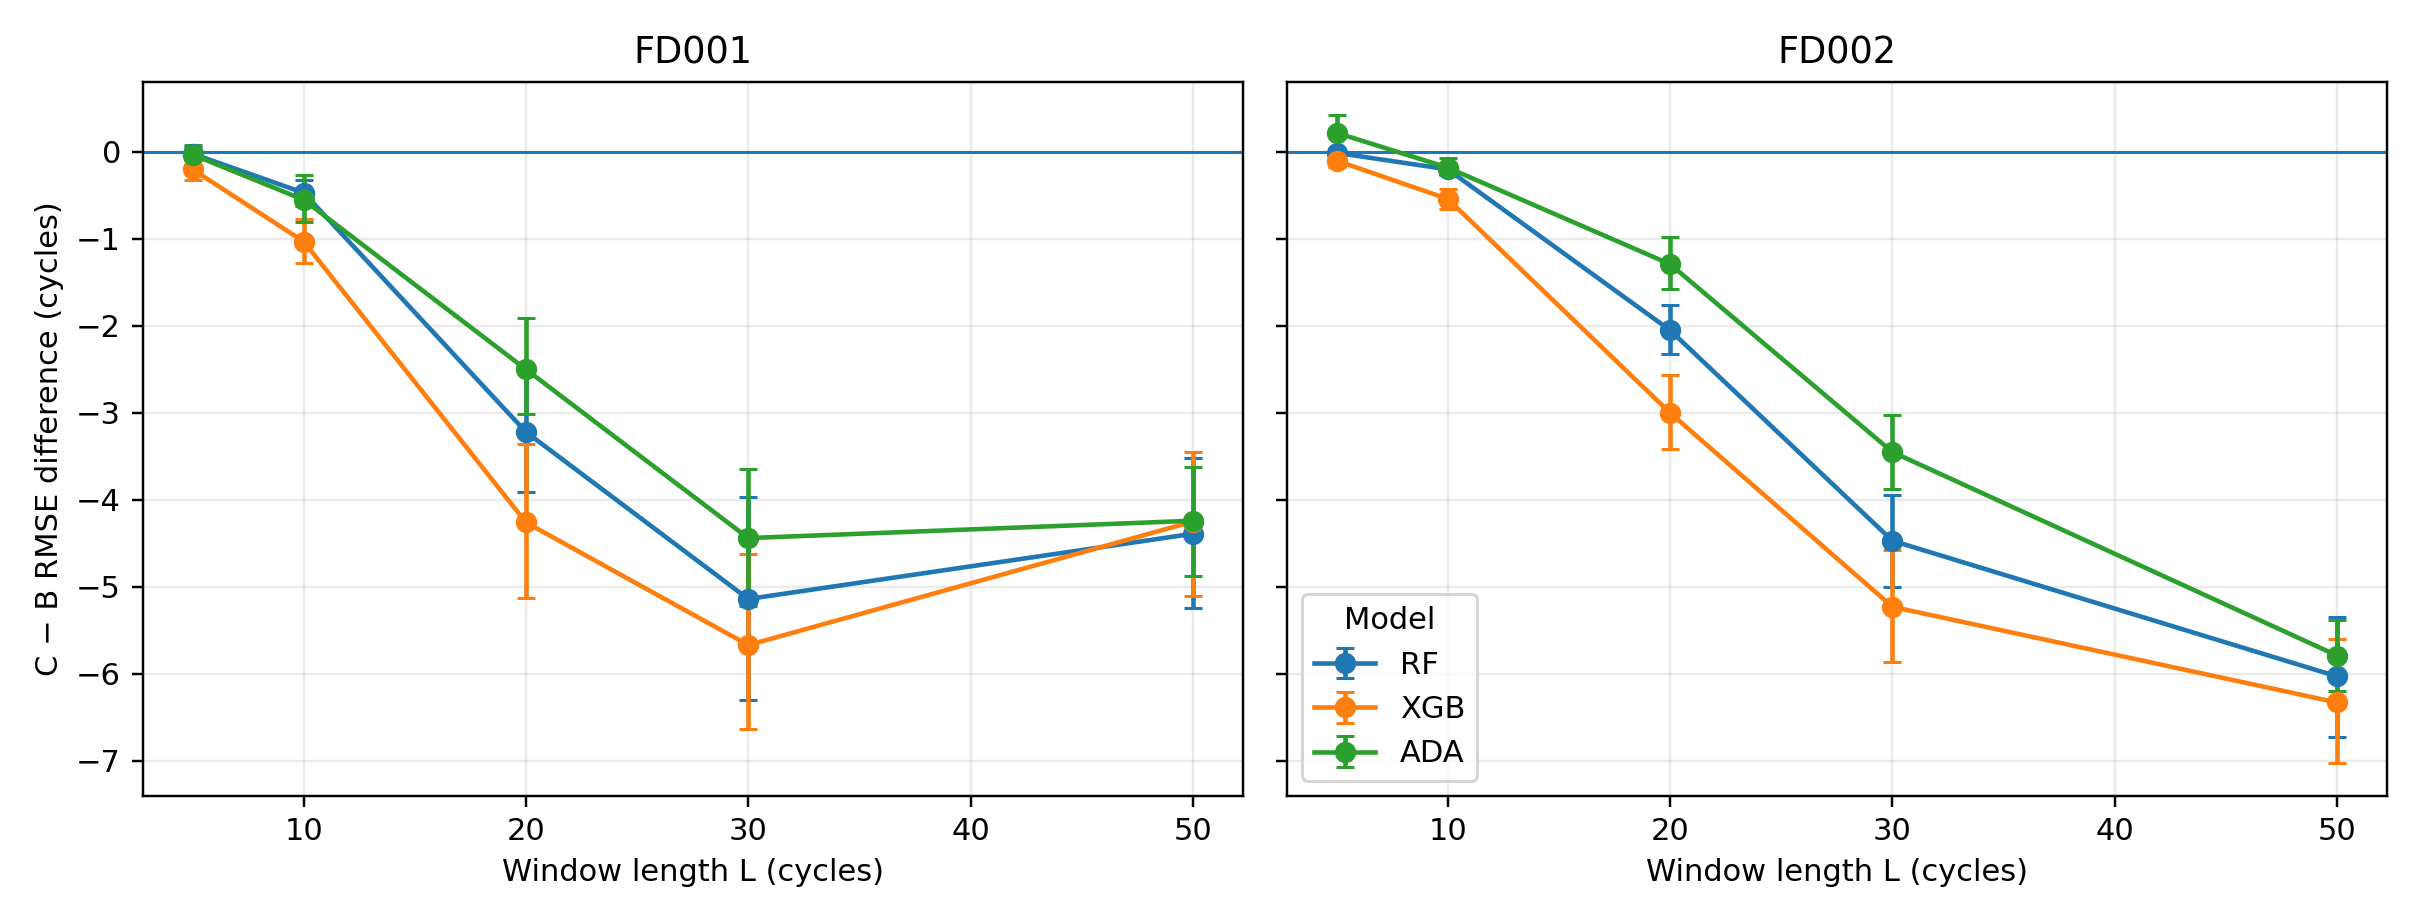
\includegraphics[width=0.86\linewidth]{figures/q1_trend_gain.png}\caption{Q1 trend contribution across window lengths. Points show C-minus-B RMSE differences and bars show the supplied 95\% engine-bootstrap intervals. Negative values indicate improvement from ordered trend features. Produced from the Q1 experiment results in \texttt{output1.ipynb}.}\label{fig:q1}\end{figure}

The shuffled condition D generally returns close to B, whereas C is better than D in all six reported model--dataset official-test comparisons. This supports the conclusion that the true order contributes information beyond the set of values in a window. It does not establish that every possible temporal representation or window length will benefit equally.

Ridge and Lasso follow the same overall Q1 pattern: condition C has the lowest official-test RMSE among A--D for both regularized models on both datasets (Table~\ref{tab:q1test}).

\subsection{Q2:}
\textbf{Answer: Yes for FD002, with preprocessing order mattering; effectively no change for FD001.} On the six-regime FD002 subset, AF produces the lowest validation and official-test RMSE for all three models. FD001 results are effectively identical across N, AF and DF, which is the expected control behaviour when there is only one operating condition.



\begin{table}[H]\centering\small
\caption{Q2 five-fold validation RMSE (mean $\pm$ standard deviation across folds), arranged by operating-condition strategy. The best model within each dataset--strategy row is identified in bold.}\label{tab:q2cv}
\begin{tabular}{ll lccc}\toprule
Dataset & Strategy & Best model & RF & XGB & ADA\\\midrule
FD001 & N (global) & \textbf{XGB} & $11.35\pm0.64$ & $\mathbf{11.23\pm0.45}$ & $12.85\pm0.47$\\
 & AF (adjust first) & \textbf{XGB} & $11.35\pm0.64$ & $\mathbf{11.23\pm0.45}$ & $12.85\pm0.47$\\
 & DF (difference first) & \textbf{XGB} & $11.34\pm0.63$ & $\mathbf{11.23\pm0.40}$ & $12.90\pm0.48$\\\midrule
FD002 & N (global) & \textbf{XGB} & $23.05\pm1.93$ & $\mathbf{22.97\pm1.99}$ & $24.76\pm1.47$\\
 & AF (adjust first) & \textbf{XGB} & $14.04\pm0.71$ & $\mathbf{13.81\pm0.72}$ & $16.13\pm0.33$\\
 & DF (difference first) & \textbf{RF} & $\mathbf{20.07\pm1.41}$ & $20.14\pm1.45$ & $21.95\pm0.62$\\\bottomrule
\end{tabular}
\end{table}

\begin{table}[H]\centering\small
\caption{Q2 official-test results, arranged by operating-condition strategy. The best model within each dataset--metric--strategy row is identified in bold. Each value is from one official test evaluation; seed-based uncertainty is unavailable for this fixed test set.}\label{tab:q2test}
\begin{tabular}{lll lrrr}\toprule
Dataset & Metric & Strategy & Best model & RF & XGB & ADA\\\midrule
FD001 & RMSE & N & \textbf{RF} & $\mathbf{13.02}$ & $13.32$ & $13.82$\\
 & & AF & \textbf{RF} & $\mathbf{13.02}$ & $13.32$ & $13.82$\\
 & & DF & \textbf{RF} & $\mathbf{13.06}$ & $13.28$ & $13.82$\\
FD002 & RMSE & N & \textbf{XGB} & $20.88$ & $\mathbf{19.44}$ & $23.45$\\
 & & AF & \textbf{RF} & $\mathbf{13.47}$ & $14.03$ & $15.47$\\
 & & DF & \textbf{RF} & $\mathbf{16.96}$ & $17.11$ & $20.12$\\\midrule
FD001 & NASA score & N & \textbf{RF} & $\mathbf{260}$ & $302$ & $272$\\
 & & AF & \textbf{RF} & $\mathbf{260}$ & $302$ & $272$\\
 & & DF & \textbf{RF} & $\mathbf{262}$ & $286$ & $272$\\
FD002 & NASA score & N & \textbf{XGB} & $2363$ & $\mathbf{1988}$ & $2652$\\
 & & AF & \textbf{RF} & $\mathbf{700}$ & $797$ & $898$\\
 & & DF & \textbf{RF} & $\mathbf{1231}$ & $1242$ & $1491$\\\bottomrule
\end{tabular}
\end{table}

\noindent\textit{Reading the tables:} N denotes global normalization, AF denotes regime adjustment before temporal feature extraction, and DF denotes raw differencing before regime-specific scaling. The ``Best model'' column explicitly names the lowest-scoring model for that row; the corresponding score is also bold. Lower RMSE and lower NASA score are better. Bold does not imply that the difference is statistically significant.

On FD002, AF improves validation RMSE over N by 39.1\% for RF, 39.9\% for XGB and 34.9\% for ADA. DF also improves over N, but is consistently worse than AF: its validation RMSE is approximately 36--46\% higher than AF, depending on the model. The official-test results show the same ordering, AF $<$ DF $<$ N. Across FD002, AF is the best preprocessing strategy for each model on both validation and official-test RMSE. The bold entries in Tables~\ref{tab:q2cv} and~\ref{tab:q2test} identify the best model within each strategy row; these model-wise minima should not be interpreted as statistically significant pairwise model rankings. Figure~\ref{fig:q2} summarizes the FD002 validation comparison.

\begin{figure}[H]\centering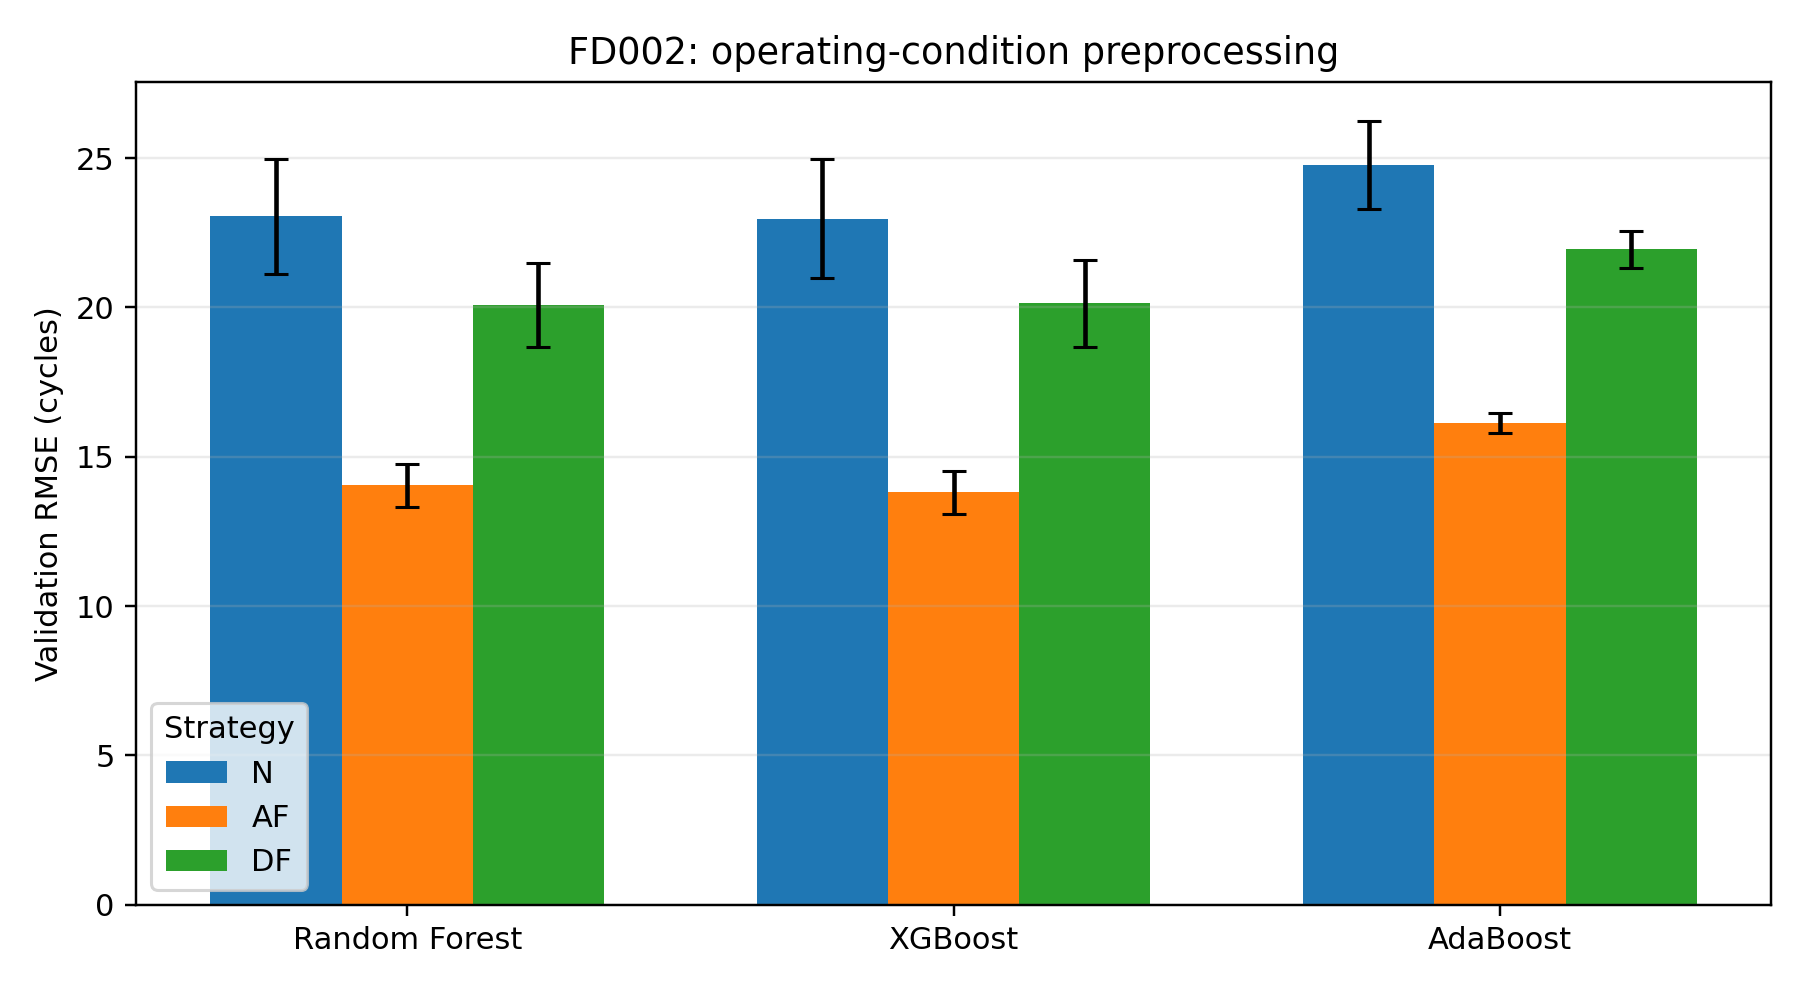
\includegraphics[width=0.88\linewidth]{figures/q2_fd002_cv.png}\caption{Q2 FD002 five-fold validation RMSE for global normalization (N), adjust-first (AF), and difference-first (DF). Error bars show fold standard deviations ($n=5$ folds). Produced from the Q2 experiment outputs in notebook \texttt{F7} with \texttt{q2\_core.py}.}\label{fig:q2}\end{figure}

The Q2 notebook reports 2,000 engine-level bootstrap repetitions. For FD002, AF-minus-N RMSE contrasts are $-9.06$ (RF; 95\% CI $[-10.04,-8.07]$), $-9.21$ (XGB; $[-10.29,-8.10]$), and $-8.66$ (ADA; $[-9.34,-7.97]$); Holm-adjusted $p=0.0045$ for each. DF-minus-AF contrasts are positive: $+6.04$ (RF; CI $[5.34,6.73]$), $+6.35$ (XGB; $[5.62,7.12]$), and $+5.83$ (ADA; $[5.41,6.27]$), again with adjusted $p=0.0045$. Thus the bootstrap evidence supports both the benefit of AF over N and the advantage of AF over DF on FD002. Under FD001, the representations are equivalent by construction because the single regime makes global and condition-specific statistics identical.

\section{Failure analysis:}
FD002 performs worst under global normalization because its six operating regimes create sensor-distribution shifts that global scaling does not remove. AF reduces this error; DF can retain regime offsets when raw differences cross regime transitions. For Q1, the current-cycle baseline A and summary/shuffled conditions B/D are weaker than C at long windows, while the trend benefit is small at $L=5$. The supplied subgroup analysis does not show a consistent concentration of benefit near failure, so we make no such claim. Finally, 7 FD001 and 24 FD002 test trajectories require left-padding to 50 cycles; the available results do not isolate their contribution to total error.
\section{Discussion and limitations:}
Q1 shows that temporal order adds information beyond window summaries, especially at longer windows. Q2 shows that condition adjustment benefits FD002, with AF outperforming DF; FD001 is a one-regime negative control.

The implemented scope addresses the two approved questions on FD001/FD002. AdaBoost was added to the Q1/Q2 tree-model comparisons, and Ridge/Lasso are included in the Q1 model comparison; the proposed mean-RUL baseline was not run. Repeated-split and early-/near-failure analyses were not fully delivered, so conclusions are limited to the reported five-fold and bootstrap evidence. The Q1 shuffle is diagnostic rather than a perfect intervention; Q2 uses one principal partition/seed, AF combines clustering with normalization, and DF is one transition-handling definition. Results show predictive associations, not physical causation or generalization to FD003/FD004. Future work should repeat partitions and inspect engine- and sensor-level residuals.
\section{Conclusion:}
For Q1, true temporal order improves RUL prediction beyond window summary statistics, particularly for longer windows: at $L=50$, the cross-validation RMSE reduction is approximately 4.2--4.4 cycles on FD001 and 5.8--6.3 cycles on FD002. For Q2, condition-specific adjustment before temporal feature extraction substantially improves prediction on multi-condition FD002, while FD001 remains effectively unchanged; adjusting first also outperforms differencing first. Together, the results support temporal structure and condition-aware preprocessing for C-MAPSS RUL prediction.

\section*{Reproducibility statement:}
The Q1 entry points are \texttt{Ordered\_vs\_Shuffled\_Window\_Experiment.ipynb} and the Ridge/Lasso implementation in \texttt{ridge-lasso-rul.ipynb}; Q2 uses \texttt{F7} with \texttt{q2\_core.py}. Run the notebooks with \texttt{jupyter nbconvert --to notebook --execute <notebook>}. The data are the NASA PCoE C-MAPSS FD001/FD002 train, test and RUL files. Q1 took about 158 minutes; Q2 fitting used CPU and Q1 recorded GPU availability for XGBoost, but exact hardware specifications were not logged. Reported Q2 models use seed 42 and 2,000 engine-level bootstrap repetitions; Ridge/Lasso uses seed 42, five engine-wise folds and shuffle seeds 101/202/303. No single tested command regenerates every table and figure: figures are notebook outputs and tables were assembled from recorded results. This is an acknowledged reproducibility limitation.
\clearpage
\section*{Contribution statement:}
The project proposal states that all members contribute equally across dataset preparation, RUL construction, temporal feature engineering, preprocessing experiments, model implementation, evaluation, analysis and report preparation. The table below records the equal overall contribution specified in the approved proposal.
\begin{center}\begin{tabularx}{\linewidth}{@{}lYr@{}}\toprule
Member & Main contributions & Share (\%)\\\midrule
Rajorshi Adhikary & Equal contribution across the project stages listed in the approved proposal & 33.3\\
Anesu Kabuku & Equal contribution across the project stages listed in the approved proposal & 33.3\\
Tanmoy Paul & Equal contribution across the project stages listed in the approved proposal & 33.4\\\bottomrule
\end{tabularx}\end{center}

\section*{AI-use summary:}
AI assistance was used to support report organization, explanation of statistical and preprocessing concepts, and consistency checks across the supplied experiment summaries. AI-generated text and interpretations were checked against the project proposal, notebooks, experiment reports, tables and recorded test outputs. Numerical results in this report are taken from the supplied project artifacts; no experimental metrics were intentionally generated by the writing assistant. The team remains responsible for verifying every result, citation, code path and contribution statement before submission.

\begin{center}\begin{tabularx}{\linewidth}{@{}lYl@{}}\toprule
Tool(s) & Used for & Verification\\\midrule
ChatGPT & Report organization, explanation and cross-checking & Compared against supplied notebooks, proposal and result PDFs\\\bottomrule\end{tabularx}\end{center}

\renewcommand{\refname}{References:}
\begin{thebibliography}{9}
\bibitem{cmapssdataset} A. Saxena and K. Goebel. \emph{Turbofan Engine Degradation Simulation Data Set}. NASA Prognostics Data Repository, NASA Ames Research Center, Moffett Field, CA, 2008. Available at: \url{https://www.nasa.gov/intelligent-systems-division/discovery-and-systems-health/pcoe/pcoe-data-set-repository/}. Accessed November 9, 2026.
\bibitem{saxena2008} A. Saxena, K. Goebel, D. Simon, and N. Eklund. Damage propagation modeling for aircraft engine run-to-failure simulation. In \emph{Proceedings of the 1st International Conference on Prognostics and Health Management (PHM)}, 2008.
\bibitem{asif2022} O. Asif, S. A. Haider, S. R. Naqvi, J. F. W. Zaki, K. S. Kwak, and S. M. R. Islam. A deep learning model for remaining useful life prediction of aircraft turbofan engine on C-MAPSS dataset. \emph{IEEE Access}, 10:95425--95440, 2022. doi:10.1109/ACCESS.2022.3203406.
\bibitem{dinten2025} R. Dint\'en and M. Zorrilla. Using time series foundation models for few-shot remaining useful life prediction of aircraft engines. \emph{Computational Modeling in Engineering \& Sciences}, 144(1), 2025. doi:10.32604/cmes.2025.065461.
\end{thebibliography}

\clearpage
\appendix
\setcounter{table}{0}\renewcommand{\thetable}{A\arabic{table}}\renewcommand{\theHtable}{A\arabic{table}}
% \section{Hyperparameters and additional results:}\label{app:additional}
% % \vspace{12pt}
% % \begin{figure}[H]
% % \centering
% % 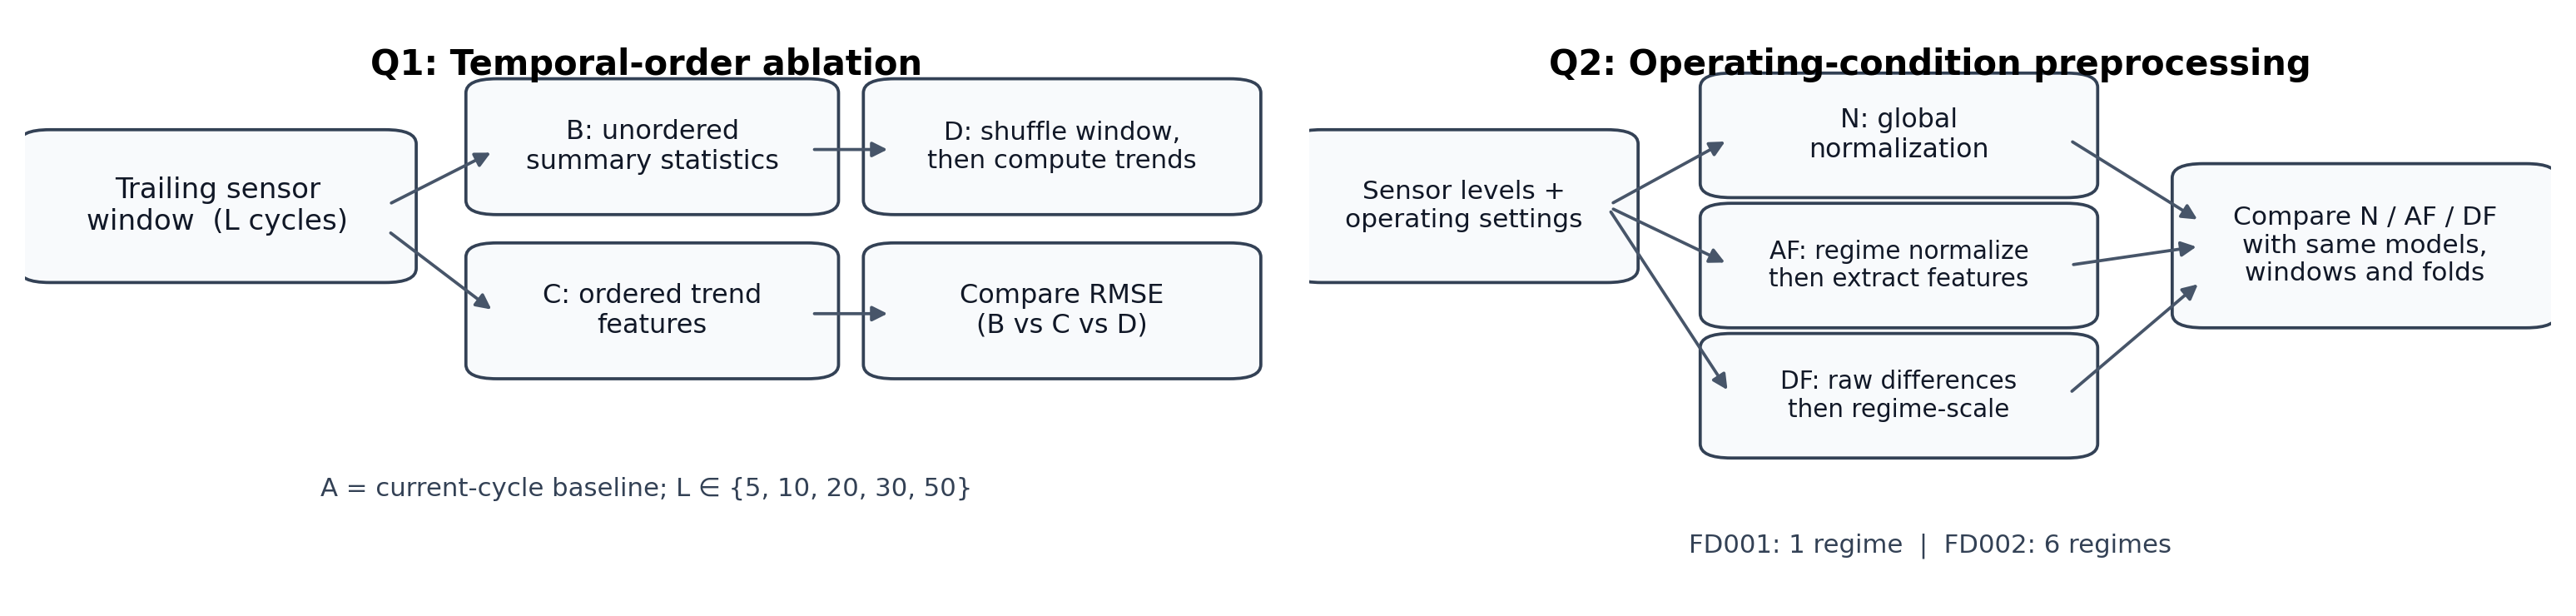
\includegraphics[width=\linewidth]{figures/methodology_workflows.png}
% % \caption{Two independent experimental pipelines. Q1 changes the temporal feature condition (A--D) and window length, then compares five model families. Q2 fixes the ordered representation and $L=50$, changes only the preprocessing strategy (N/AF/DF), and compares RF, XGB and ADA. The Q1 conditions are not stages of Q2, and the Q2 strategies are not additional Q1 conditions.}
% % \label{fig:method-workflows}
% % \end{figure}
% \subsection{Regularized linear objectives:}
% For standardized feature vector $\mathbf{x}_i$, Ridge and Lasso minimize the squared-error objectives with $L_2$ and $L_1$ penalties, respectively:
% \[
% \widehat{\boldsymbol\beta}_{R}=\arg\min_{\boldsymbol\beta}\left\{\sum_{i=1}^{N}(y_i-\mathbf{x}_i^T\boldsymbol\beta)^2+\lambda\|\boldsymbol\beta\|_2^2\right\},
% \]
% \[
% \widehat{\boldsymbol\beta}_{L}=\arg\min_{\boldsymbol\beta}\left\{\sum_{i=1}^{N}(y_i-\mathbf{x}_i^T\boldsymbol\beta)^2+\lambda\|\boldsymbol\beta\|_1\right\}.
% \]
% The penalties are fixed at the notebook values (Ridge $\alpha=1.0$; Lasso $\alpha=0.01$); no penalty search is claimed.



% Ridge and Lasso are part of the Q1 model comparison and are reported alongside RF, XGB and ADA in Table~\ref{tab:q1test}. Their fixed penalties and fold-fitted feature standardization are documented in the Methodology section.

% The team also exchanged references to two additional notebooks, \texttt{fd001-impactfull-feature-extraction.ipynb} and \texttt{fd002-impactfull-feature-extraction.ipynb}, as possible supplementary experiments. The available communication screenshot confirms the notebook names and that they were considered for a supplementary section, but it does not contain methods, outputs or numerical results. Their results are therefore not represented as completed evidence in this report. They should be added only after the notebook files and their outputs have been reviewed and the analysis can be reproduced. The screenshot itself is not included as a scientific figure because a chat exchange is not experimental evidence.

% The separate feature-budget notebooks are exploratory analyses and are not substituted for the two primary question-wise experiments. In FD001, 54 of the 189 extracted AF features had zero variance, leaving 135. The 60-feature budget gave the lowest reported validation RMSE for both RF (11.172) and XGB (11.160), with official-test RMSE 12.844 and 13.043, respectively. In FD002, zero-variance removal left 189 features for N, 175 for AF and 179 for DF. Under AF, the 60-feature budget gave validation RMSE 13.765 (RF) and 13.641 (XGB), and test RMSE 13.335 and 13.597. These exploratory results suggest that a compact ranked subset can retain much of the predictive signal; they are reported separately because this feature-budget experiment changes the representation and should not be conflated with the fixed-feature Q2 ablation.

% The Q1 notebook includes explicit checks that: the NASA score penalizes late predictions more heavily; the RMSE implementation is correct; computed slopes agree with a linear-fit reference; engine folds cover each engine exactly once; cut-off cycles are at least 50; windows end at the current cycle and do not use future observations; shuffling leaves order-invariant statistics unchanged while altering temporal descriptors; and scored rows are consistent across window lengths. The notebook records 152,075 engine-level result rows and a full experiment runtime of approximately 158 minutes.

% The Q2 notebook verifies that N, AF and DF feature representations are identical on FD001 and differ on FD002; windows use no future observations; engine-boundary differences are handled; the DF path reconstructs its last-minus-first change; training and test feature construction are consistent; short test sequences are padded; the five folds contain 20 validation engines each for FD001 and 52 each for FD002; and temporal slopes agree with a linear-regression calculation. It also reloads three representative saved models and confirms that their predictions reproduce the stored test predictions. The experiment reports 18 saved model bundles (two datasets, three preprocessing strategies and three models).


% \clearpage
% \section{Selected notebook execution evidence}
% The following panels reproduce selected saved outputs from the team's F-series notebooks. They are supplementary evidence and do not replace the notebooks or imply a new experiment run during report preparation.

% \begin{figure}[H]\centering
% 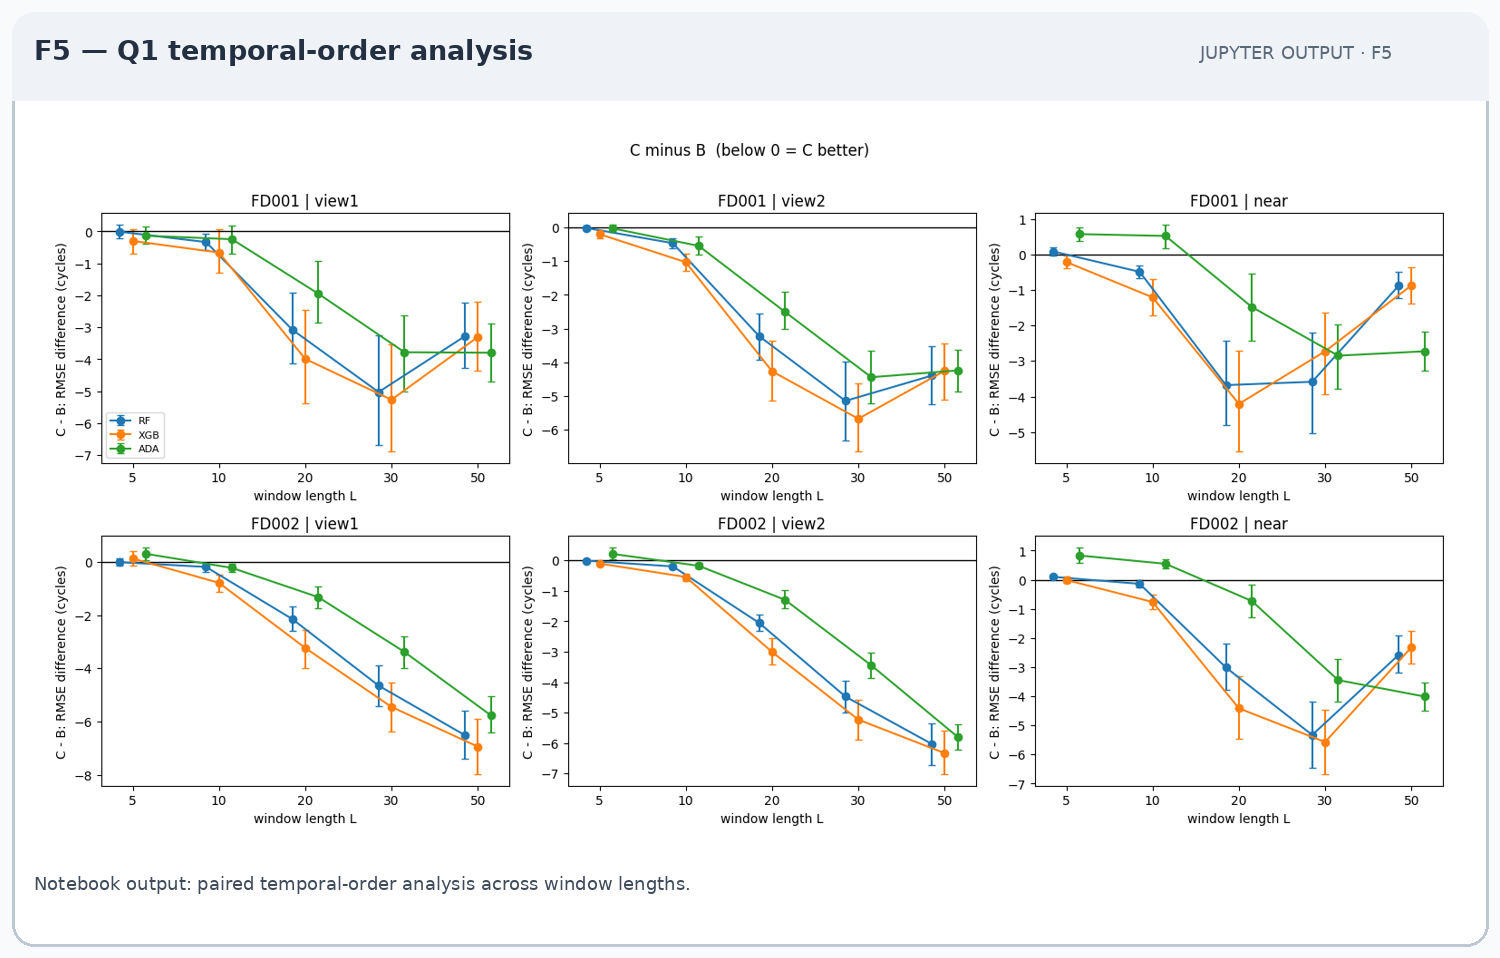
\includegraphics[width=0.96\linewidth,height=0.72\textheight,keepaspectratio]{figures/notebook_evidence_1.png}
% \caption{F5 notebook output: Q1 temporal-order analysis.}
% \end{figure}

% \begin{figure}[H]\centering
% 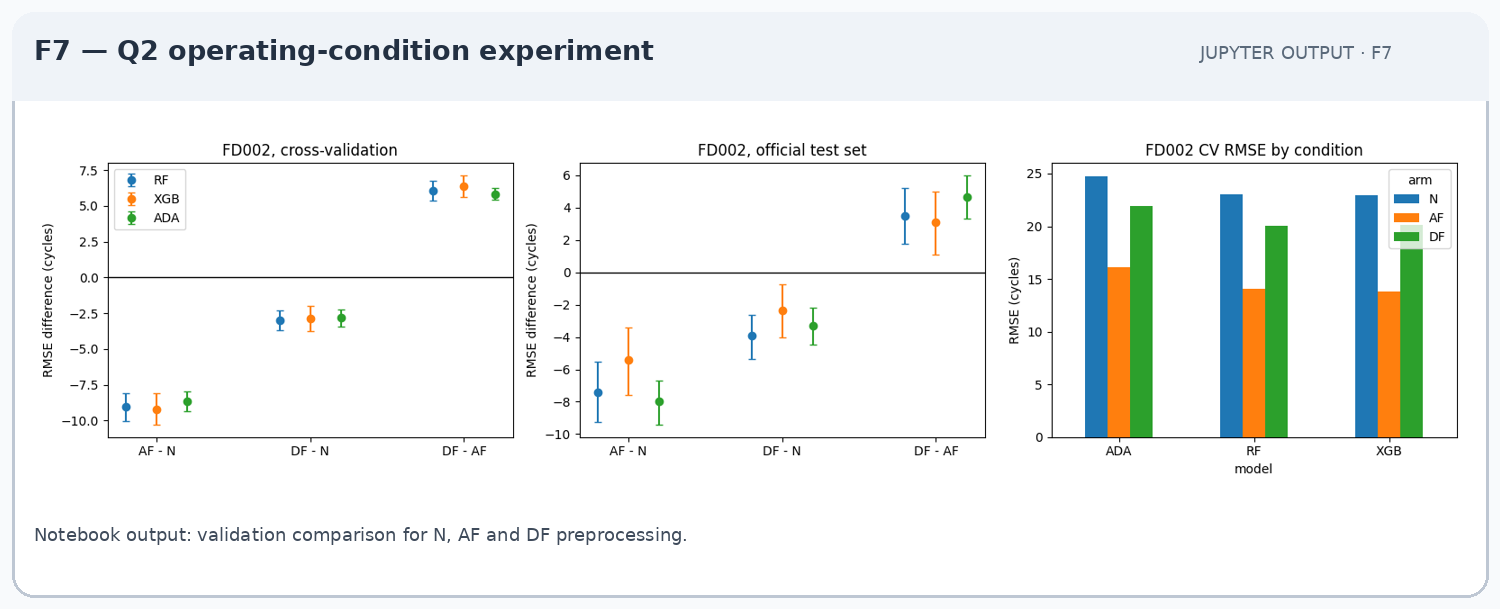
\includegraphics[width=0.96\linewidth,height=0.72\textheight,keepaspectratio]{figures/notebook_evidence_2.png}
% \caption{F7 notebook output: Q2 paired contrasts and RMSE by preprocessing condition.}
% \end{figure}

% \begin{figure}[H]\centering
% 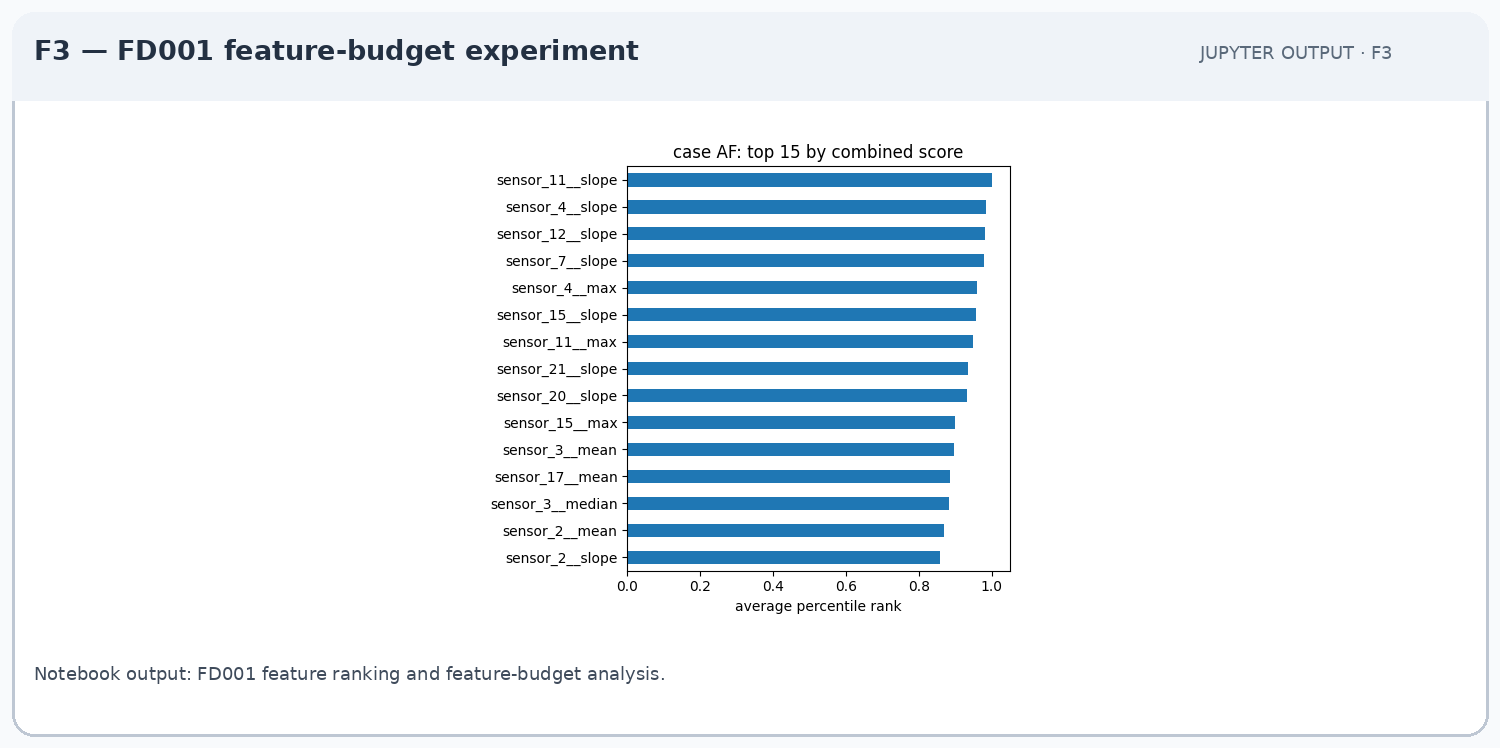
\includegraphics[width=0.96\linewidth,height=0.72\textheight,keepaspectratio]{figures/notebook_evidence_3.png}
% \caption{F3 notebook output: FD001 feature-budget analysis.}
% \end{figure}

% \begin{figure}[H]\centering
% 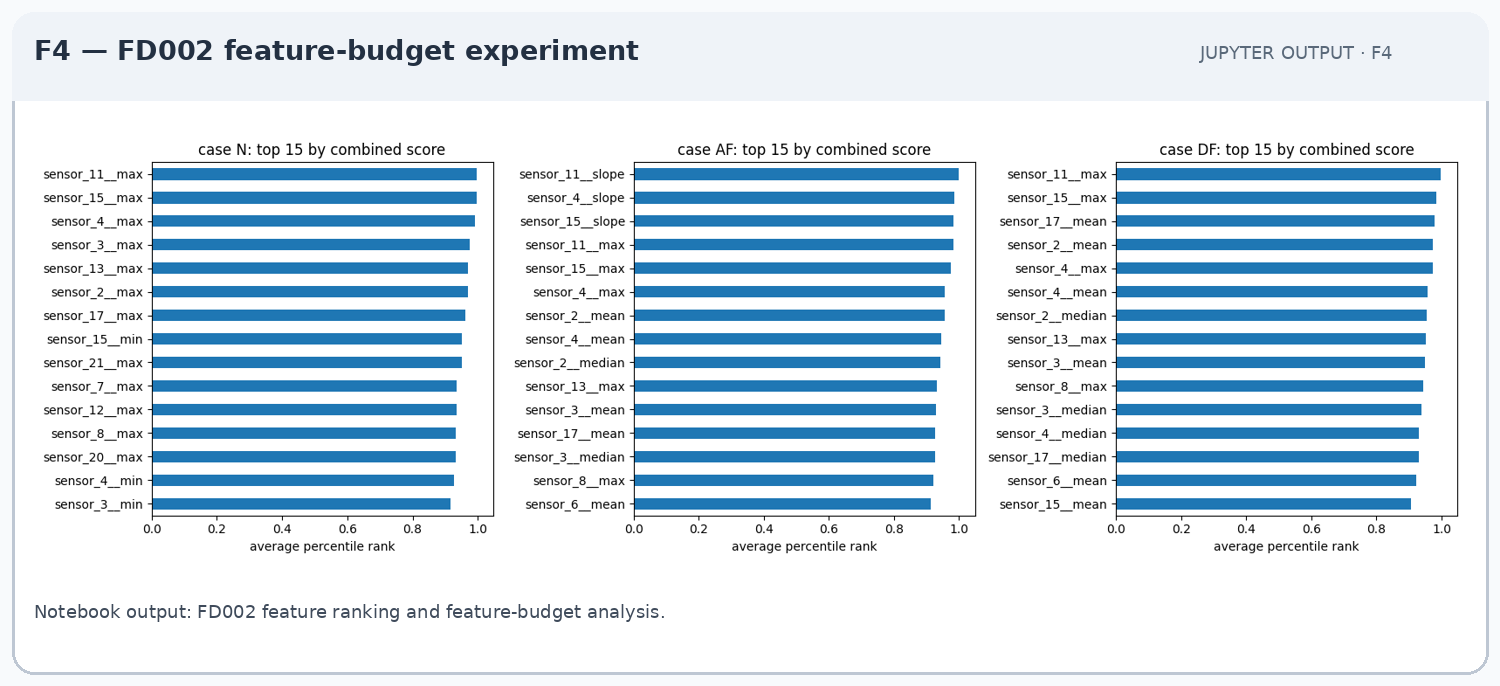
\includegraphics[width=0.96\linewidth,height=0.72\textheight,keepaspectratio]{figures/notebook_evidence_4.png}
% \caption{F4 notebook output: FD002 feature-budget analysis.}
% \end{figure}

\end{document}
